% Chapter 1

\chapter{Introduction} 
\label{chap:introduction} 

As the college drop-out brother of a double PhD academic sister, I grew up embracing and developing an interest-driven, non-academic way of learning and participating in the world. I was determined to learn through interacting, and through practice with intellectuals and practitioners as my peers and mentors. I focused my energy on being a connector of ideas and people and supporting organizations that I believed were having an impact on the world --- a sort of public intellectual and activist.

When I joined the Media Lab as its director seven years ago, its impact-oriented research and the unstructured innovation thus felt familiar and consistent with my own values and practice. As Miles's Law \cite{miles1978origin} states, ``Where you stand depends on where you sit.'' While the Media Lab is free of many of the constraints of disciplinary scholarship, we are part of an academic institution and are necessarily academic in our degree programs and in our faculty promotion process. Since my arrival, I've become more familiar with and respectful of disciplines and academic rigor. Having said that, I believe it is my role and the role of the Media Lab to develop a new model of rigor and how an academic institution contributes to the world.

I am accidentally approaching the process backwards, having becoming Lab director first, then a professor of the practice and now a PhD candidate, but this has given me the advantage of looking at everything from roughly the opposite direction than is typical. One of the motivations for writing this dissertation is to better understand the process of putting together a dissertation. This understanding has already helped me better comprehend the dynamics of being a student and the process of producing and defending claims much better.

In this dissertation, I make broad claims and suggest a way forward for the Media Lab and myself. I connect to existing work and literature from across many disciplines, but I am not a dedicated researcher in any one discipline, and my depth is limited compared to specialists in any of these fields. My purpose is to draw on and connect these disciplines and to develop and propose a new way to work across and between disciplines.

\marginpar{Some would argue that the world is happier and more fair \cite{pinker_better_2012}, while others would argue that much of this abundance is a result of exploitation and extraction that is neither fair nor sustainable and that leads to global instability and conflict \cite{cronin2009exploiting}.}As a connector and a person focused on the synthesis of ideas and practice, the majority of my work is by definition collaborative and mostly in support of the work of others. In this dissertation, I describe this at a meta layer, and argue that what I have learned through the practice of my work informs my ideas about a new theory, as well as practical methods for understanding and intervening.

We are in a pivotal moment in history where the problems that now face civilization are fundamentally different from the challenges of the past. The Media Lab is playing an important role in addressing these challenges. This dissertation is about what our role is and how we can increase its positive impact.

Advances in science and technology enabled the industrial revolution that allowed civilization to scale and prosper by making the world more efficient, effective, and rich. Some would argue that the world is happier and more fair \cite{pinker_better_2012}, while others would argue that much of this abundance is a result of exploitation and extraction that is neither fair nor sustainable and that leads to global instability and conflict \cite{cronin2009exploiting}.

The problems to which we have applied our academic and business efforts have created benefits to society such as material abundance, the elimination of acute medical problems, and overall convenience and efficiency. At the same time, systems of government and markets have developed that have made the deployment of capital extremely efficient and effective for capitalists.

Society has developed a number of tools, including: entrepreneurship and a way to attract capital to companies to pursue exponential growth; technical tools to improve efficiency and productivity in the capital markets; infrastructure; drugs to increase life expectancy; and educational and vocational systems that support physical and economic mobility. For the first time, however, we are seeing a decrease in life expectancy in the United States \cite{kmxa17}, attributed to the opioid crisis \cite{LifeExpe48:online}. Chronic disease continues to be a problem in the US and is increasingly a problem in many other countries caused by the very abundance and convenience we created, which have led to overeating and a lack of exercise, as well as drug abuse. There has been a drop in physical and economic mobility in the United States, a decline in public understanding of science and math \cite{noauthor_internationally_nodate}, and increasing income disparity \cite{alston_statement_2017}. Yet we continue to use the tools that have caused our current problems to solve our new problems. Donella Meadows, a systems dynamics researcher who worked at MIT and whose work has had a deep impact on my thinking, points out in ``Leverage Points: Places to Intervene in a System'' \cite{meadows_leverage} that we are trying to solve the problems of environmental destruction, poverty and hunger with growth when these problems are themselves a byproduct of growth. 

\marginpar{We must address our new generation of complex problems --- climate change, social disparity and polarization, poor health --- in new ways that not only require new tools but a paradigm shift away from the dominant values that have developed through the industrial revolution.}We must address our new generation of complex problems --- climate change, social disparity and polarization, poor health --- in new ways that not only require new tools but a paradigm shift away from the dominant values that have developed through the industrial revolution. As Scott E. Page explores in \textit{Diversity and Complexity} \cite{page2010diversity}, adaptive attributes of such complex systems can be harnessed to direct the systems towards sustainable and flourishing states.
% * <david@weinberger.org> 2018-06-27T23:37:12.082Z:
% 
% The standard understanding of eudaimonia doesn't match well with raison d'etre. I'd drop the French reference, just to be safe. Eudaimonia for Aristotle has more to do with leading a good life, which entails pursuing excellence in one's activities (= the Greek idea of "virtue"), moderation in all, being healthy, and avoiding being captured and made into a slave. It also helps not to be disabled or ugly. (That's Aristotle speaking, not me.) Fisher talks about "flourishing," which is a good way of encapsulating the concept.
% 
% ^.

William Fisher, a Professor at Harvard Law School, in ``Theories of Intellectual Property'' \cite{fisher2001theories} describes many ways of thinking about human flourishing. The definition of flourishing that I am using to describe healthy systems to is similar to the ``eudaimonia'' and productive self-actualization described by Aristotle in ``Nicomachaen Ethics`` \cite{rowe2002nicomachean}. This is also similar to the Japanese term \begin{CJK}{UTF8}{min}生き甲斐\end{CJK} \textit{Ikigai} or the French term \textit{raison d'être}, which describe a meaning for living. A shift in priorities towards a more eudaimonic notion of flourishing over a hedonistic one is a key part of the paradigm shift I believe we need.

It is clear all that complex systems are interconnected and must be viewed together, and that there are many similarities in how we might intervene in these different systems to increase flourishing in the form of resilience and robustness. The industrial paradigm of control and compositional thinking\footnote{Neri Oxman often refers to the notion that something is just the sum of its parts or that a complex system can be disassembled and understood to be ``compositional thinking.''} are no longer appropriate.
 
The Internet and communications technology have significantly decreased the cost of collaboration and communication and increased complexity. Before the industrial revolution, most production occurred in markets. With the industrial revolution came corporations that increased efficiency through centralization of resources and management \cite{coase_nature_1937}. The Internet brought commons-based peer production --- non-corporate production modes that allowed participants to assign their own labor with a more decentralized and bottom-up organization structure \cite{benkler_coases_2002}. (See figure \autoref{fig:internetcomplex}.)

\begin{figure}[t]
 \centering
 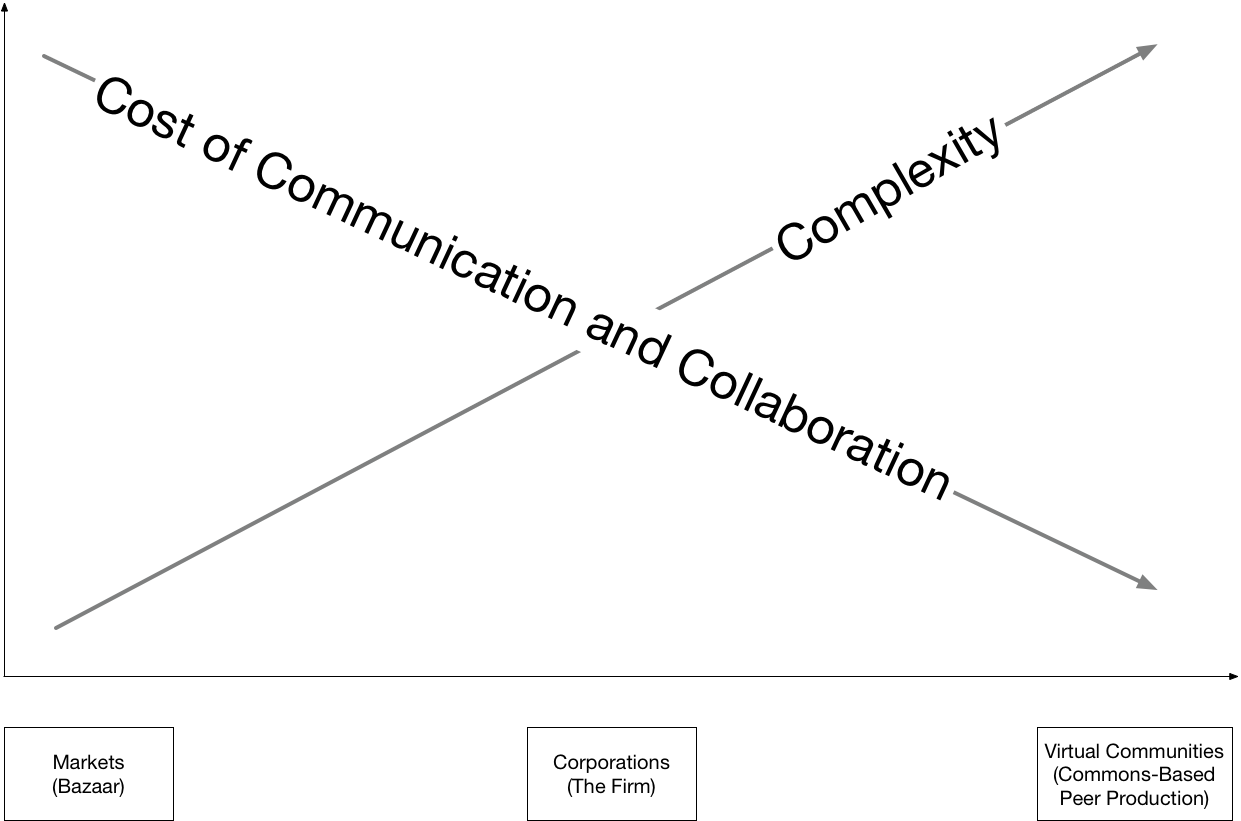
\includegraphics[width=1\textwidth]{pictures/TheInternetMarkets}
 \caption[The Internet decreased collaboration and communication costs and increased complexity.]{The Internet and communications technology have significantly decreased the cost of collaboration and communication and increased complexity. Before the industrial revolution, most production occurred in markets. With the industrial revolution came corporations that increased efficiency through centralization of resources and management \cite{coase_nature_1937}. The Internet brought commons-based peer production - non-corporate production modes that allowed participants to assign their own labor with a more decentralized and bottom-up organization structure \cite{benkler_coases_2002}.}
 \label{fig:internetcomplex}
\end{figure}

Corporations continued to aggregate power, distribution, and capital, prompting a regulatory intervention in the United States ; the Sherman Antitrust Act was enacted to break up monopolies that were exerting complete control over the market \cite{ShermanA12:online}. The Internet, in many ways, led to even more decentralization and the creation of more competitive and dynamic markets where once monolithic telecommunications companies had dominated. However, twenty years in to the widespread rise of the Internet, companies such as Google and Facebook are now exhibiting monopoly-like scale and behavior. This new era of monopolies is built on digital networks rather than physical goods and distribution. (See figure \autoref{fig:netmonopoly}.)

\begin{figure}[t]
 \centering
 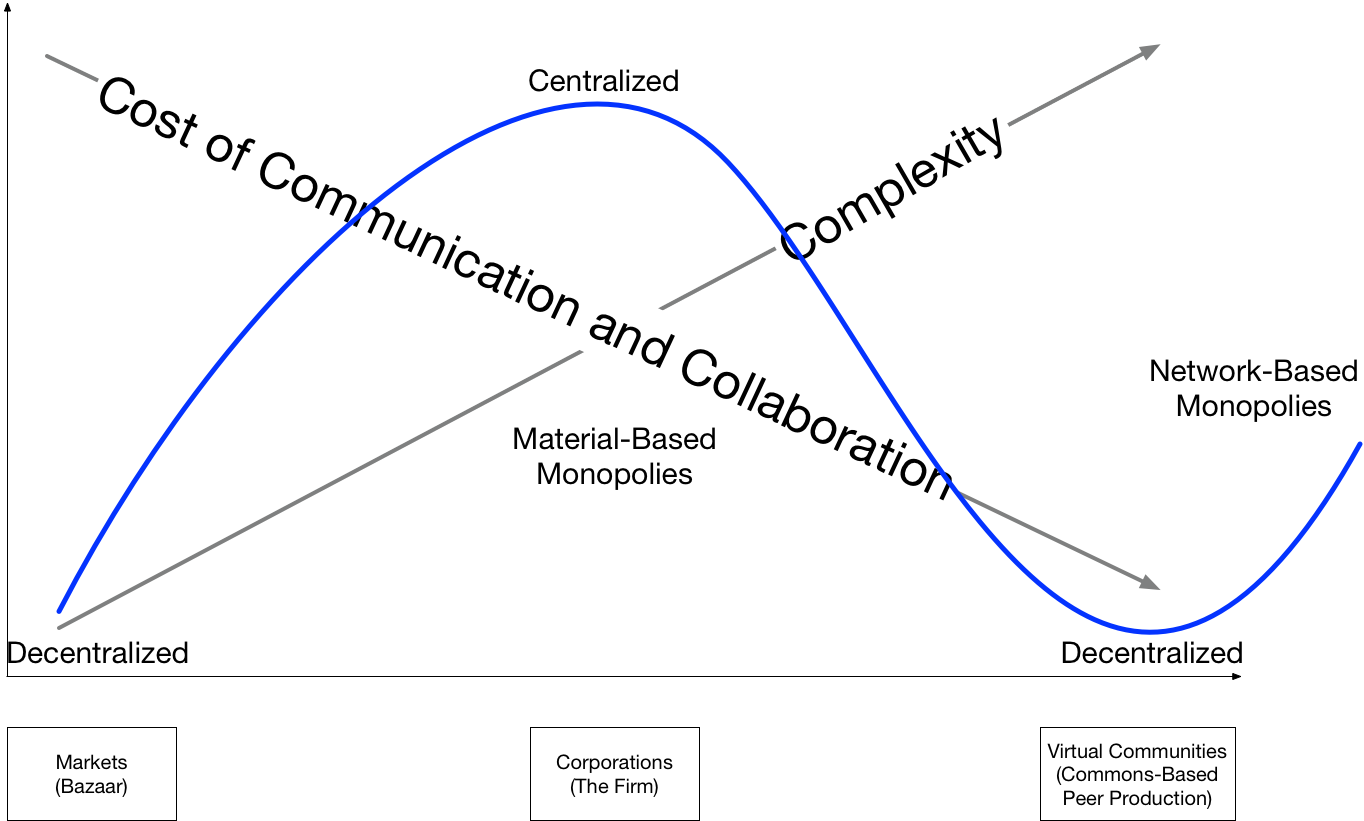
\includegraphics[width=1\textwidth]{pictures/TheInternetMarkets2}
 \caption[The Internet decentralized some monopolies but created new network-based monopolies.]{The Internet caused an unbundling of power and decentralization further diminishing the power of traditional monopolies such as telephone companies, but heralding a new generation of network-based monopolies in contrast to the material-based monopolies of the industrial revolution.}
 \label{fig:netmonopoly}
\end{figure}

The Internet has enabled organizations and movements to emerge in decentralized and bottom-up ways, but the nature of networks has also created a new kind of monopoly and centralization. These new monopoly-like enterprises have similar dynamics to the previous generation of monopolies. Our challenge is to use our new forms of organization and intervention to fight against these new forms of centralization as well as the old --- a post-Internet, community-based approach. We need to shift the paradigm of society from its orientation toward short-term capital to long-term flourishing, so that organizations and individuals can change their behavior, and the systems can evolve to become more robust and healthier.

In this dissertation, I describe the problems that must be addressed, present a theory of change, and explore concrete examples based on decades of practice. I present both a theoretical framework and practical approach for how we may transform society to address the complex problems we face today.

\section{Overview of Dissertation}
\label{intro:overview}

\begin{figure}[t]
 \centering
 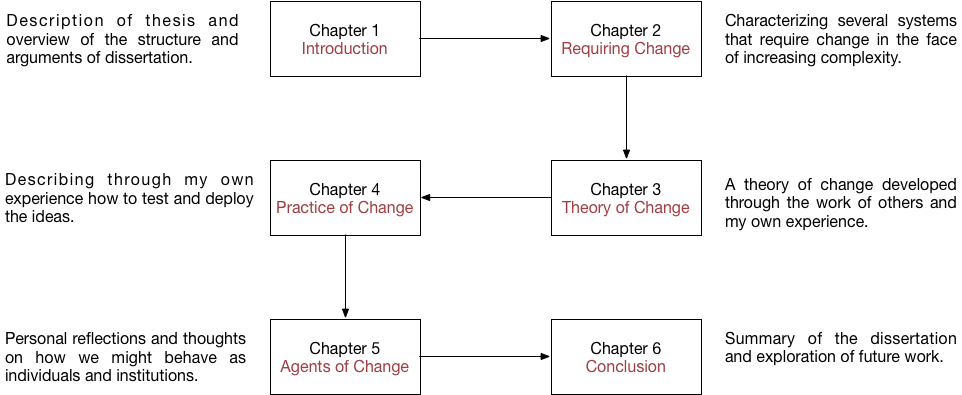
\includegraphics[width=1\textwidth]{pictures/thesisStructure2}
 \caption[Thesis Structure]{Thesis Structure: \textbf{\textit{Chapter~1}} describes the thesis and provides an overview of the structure and arguments of dissertation. \textbf{\textit{Chapter~2}} Characterizing several systems that require change in the face of increasing complexity. \textbf{\textit{Chapter~3}} presents theory of change developed through the work of others and my own experience. \textbf{\textit{Chapter~4}} includes personal reflections and thoughts on how we might behave as individuals and institutions. Finally, I end with a conclusion and an exploration of future work in \textbf{\textit{Chapter~5}}.}
 \label{fig:structure}
\end{figure}


The dissertation begins by describing five primary problem: the peril of silos; the problem of monolithic and centralized systems; the opportunity and need to rethink democracy in the post-Internet era; the need to rethink health and medicine; and how to address climate and environmental issues in \autoref{chap:requiring}.

In \autoref{chap:theory} I present a framework for understanding the systems we will be discussing. I draw on systems dynamics, evolutionary biology, cybernetics, design, history and philosophy of science, the history of the Internet, and lessons from Lawrence Lessig. I share my own thoughts on the nature of the Internet and the perils of reductionist thinking. I argue that the only way to change the system is through a paradigm shift in theories and methods of change. I argue that the intervention is best delivered through an artistic and cultural intervention, using the hippie movement as an example.

In \autoref{chap:practice} I describe how the Media Lab works, using several of the initiatives at the Media Lab as examples of an ``antidisciplinary'' approach to address the peril of silos. I then share my work as the CEO of Creative Commons, a board member of The Open Source Initiative, my work in the cryptocurrency communities since the 1990s, and my work in the venture and venture capital community to describe my learnings from, and contributions to, decentralized architectures. I share my work on various layers of the Internet infrastructure, including my role in the development of social media and the new public sphere, and my teaching and research in the ethics and governance of artificial intelligence. I consider these as contributions to reinventing the new post-Internet democracy. I discuss my course, ``Principles in Awareness'' at the Media Lab that I teach with the Venerable Tenzin Priyadarshi that explores self-awareness. I describe the Health 0.0 initiative --- a new intervention to think about the future of health and medicine, and whether we can apply learnings from the Internet and the antidisciplinary approach. I also describe my work as the board chair of PureTech Health --- a new kind of biomedical company. Lastly, I describe my work on the environment, describing the citizen radiation measurement organization Safecast as an example not only of environmental activism but as a new way of using post-Internet organizational principles to create grassroots activity. I also share the efforts of the Nia Tero organization to protect the environment through collaboration with indigenous people and local communities.

In \autoref{chap:agent} I reflect on my own journey and address some of the questions that were raised during the dissertation defense and in feedback from the committee. I discuss happiness, conviviality, interest-driven learning, and how we might as individuals and organizations apply the lessons developed through the course of this dissertation.

\autoref{chap:conclusion} is a conclusion in which I reflect on my work experience and examine my successes and failures in the form of learnings and insights. I discuss what questions remain, and conclude with a direction for my future work based on a theory of change: a fundamental, normative shift in society away from the pursuit of growth for growth's sake. I argue that this new sensibility should draw on historical trends, indigenous sensibilities, and new values emerging from the environment created by new technologies and understanding of science.
